\subsection{反例}\label{src:C.7.3-subsection}
我们给出不满足 Artin 公理的非代数层与叠的例子.
\begin{example}[模的自同构]\label{src:C.7.11}
对环 $A$ 上的模 $M$, 考虑
\[
\underline{\Aut}_A(M):\Sch/A\to\mathrm{Sets},\qquad S\mapsto\Aut_S(M\otimes_AS).
\]
若 $M$ 平坦且有限表现, 则 $\underline{\Aut}_A(M)$ 可由群概形表示 (事实上是有限型仿射群概形). 若 $M$ 不平坦或不有限表现, 则此结论不成立. 例如, 若 $A=\Bbbk$, $V=\bigoplus_{n\in\mathbb N}\Bbbk\cdot\langle e_i\rangle$, 则 $\underline{\Aut}_{\Bbbk}(V)$ 不保持极限: 令 $B=\Bbbk[x_1,x_2,\ldots]=\bigcup_nB_n$, 其中 $B_n=\Bbbk[x_1,\ldots,x_n]$, 则由 $e_i\mapsto e_i+x_{i+1}e_{i+1}$ 定义的 $V\otimes_{\Bbbk}B$ 的 $B$-自同构, 对任何 $n$ 都不由 $V\otimes_{\Bbbk}B_n$ 的 $B_n$-自同构诱导, 即 $\operatorname{colim}_n\Aut_{B_n}(V\otimes_{\Bbbk}B_n)\to\Aut_B(V\otimes_{\Bbbk}B)$ 不满射.

另一方面, 令 $A=\Bbbk[x]$, $M=A/(x)=\Bbbk$. 假设 $G=\underline{\Aut}_{\Bbbk[x]}(\Bbbk)$ 可由代数空间表示. $G\to\Spec\Bbbk[x]$ 的截面对应于 $\Aut_{\Bbbk[x]}(\Bbbk)=\Bbbk^\times$. 两个不同截面必须限制为 $\Spec\Bbbk[x]_x$ 上的不同截面, 但这与 $G$ 在 $\Spec\Bbbk[x]_x$ 上限制为平凡群概形矛盾. 层 $G$ 不满足公理 $(\mathrm{AA}_4)$ 中的强齐性条件 $(\mathrm{RS}_4^*)$. 事实上, 它不满足 Rim--Schlessinger 条件 $(\mathrm{RS}_2)$ (等价地, Schlessinger 条件 $(\mathrm H_2)$): $G(\Bbbk[\epsilon]\times_{\Bbbk}\Bbbk[\epsilon])\to G(\Bbbk[\epsilon])\times_{G(\Bbbk)}G(\Bbbk[\epsilon])$ 不是双射, 其中 $\Bbbk[\epsilon]$ 经由 $x\mapsto\epsilon$ 具有 $\Bbbk[x]$-代数结构. 事实上, $G(\Bbbk[\epsilon])=\Aut_{\Bbbk[\epsilon]}(\Bbbk)=\Bbbk^\times=G(\Bbbk)$, 而
\[
G(\Bbbk[\epsilon]\times_{\Bbbk}\Bbbk[\epsilon])=\bigl(\Bbbk[\epsilon]\times_{\Bbbk}\Bbbk[\epsilon]/(\epsilon,\epsilon)\bigr)^\times\cong\Bbbk[\epsilon]^\times\cong\Bbbk^\times\times\Bbbk.
\]
\end{example}
\begin{example}[拟凝聚层叠与非平坦凝聚层叠]\label{src:C.7.12}
若 $X$ 为域 $\Bbbk$ 上的固有概形, 则预叠 $\underline{\QCoh}(X)$ 不是代数叠, 其中其在 $S$ 上的对象为 $S$ 上平坦的拟凝聚层 $F$. 前例说明 $\underline{\QCoh}(X)$ 不保持极限 (因为相应函子甚至不全忠实), 且对角不可表, 即 $(\mathrm{AA}_1)$ 与 $(\mathrm{AA}_2)$ 均不成立. 类似地, 有限表现 (但未必平坦) 拟凝聚层的叠也不是代数叠, 且不保持极限. 由前例, $(\mathrm{AA}_2)$ 及 $(\mathrm{AA}_4)$ 的全忠实性均不成立.
\end{example}
\begin{example}[概形的自同构]\label{src:C.7.13}
若 $X$ 为 $\Bbbk$ 上的概形, 考虑
\[
\underline{\Aut}(X):\Sch/\Bbbk\to\mathrm{Sets},\qquad S\mapsto\Aut_S(X_S).
\]
若 $X$ 固有, 则它可由代数空间表示. 缺少固有性时, 此结论可能不成立. 例如, $\underline{\Aut}(\mathbb A^1)$ 不可表, 且不满足 $(\mathrm{AA}_3)$: 若 $\xi=\{\mathrm{id}\}\in\underline{\Aut}(\mathbb A^1)(\Bbbk)$, 则由命题 \bookref{C.2.4}, 切空间 $\operatorname{Def}_{\xi}(\Bbbk)$ 与 $\mathrm H^0(\mathbb A^1,T_{\mathbb A^1})=\Bbbk[x]$ 等同.
\end{example}
\begin{example}[所有代数空间的叠]\label{src:C.7.14}
设 $\mathcal X$ 为 $\Sch/\Bbbk$ 上的预叠, 其在 $\Bbbk$-概形 $S$ 上的对象为代数空间的态射 $X\to S$, 态射 $(X\to S)\to(X'\to S')$ 为笛卡尔图. 它是 $(\Sch/\Bbbk)_{\text{ét}}$ 上的叠, 但不保持极限, 且对角 $\mathcal X\to\mathcal X\times\mathcal X$ 不可表, 即 $(\mathrm{AA}_1)$ 与 $(\mathrm{AA}_2)$ 均不成立. 它也不满足 $(\mathrm{AA}_{2'})$, 因为 $\operatorname{Aut}_{\xi}(\Bbbk)$ 可能为无限维, 如前例所示.
\end{example}
\begin{example}[K3 曲面的叠]\label{src:C.7.15}
$(\Sch/\Bbbk)_{\text{ét}}$ 上的模叠 $\mathcal K_3$ 不是代数叠, 其中其在 $\Bbbk$-概形 $S$ 上的对象为代数空间的光滑固有态射 $\mathcal X\to S$, 每个纤维均为 K3 曲面. 它不满足有效性公理 $(\mathrm{AA}_5)$; 见注记 \bookref{C.5.9}.
\end{example}
现在描述 \cite{Art69c} 中 Artin 的反例. 每个例子的设定均为仿射概形的归纳系统
\[
X_1\to X_2\to X_3\to\cdots,\qquad X_q=\Spec A_q,
\]
并考虑函子
\[
\begin{aligned}
\operatorname{colim}X_q:\operatorname{AffSch}/\Bbbk&\to\mathrm{Sets}\\
\Spec R&\mapsto\operatorname{colim}\operatorname{Mor}_{\Bbbk}(\Spec R,X_i),
\end{aligned}
\]
其中 $F(R)$ 的元素为一对 $(q,\phi:A_q\to R)$ 的等价类, $q$ 为正整数, $\phi$ 为 $\Bbbk$-代数同态, 且 $(q,\phi)\sim(q',\phi')$ 当且仅当存在 $Q\geq q,q'$, 使 $A_Q\to A_q\xrightarrow\phi R$ 与 $A_Q\to A_{q'}\xrightarrow{\phi'}R$ 一致.

\bookfiguretarget{C.7.16}
\begin{figure}[htbp]
\centering
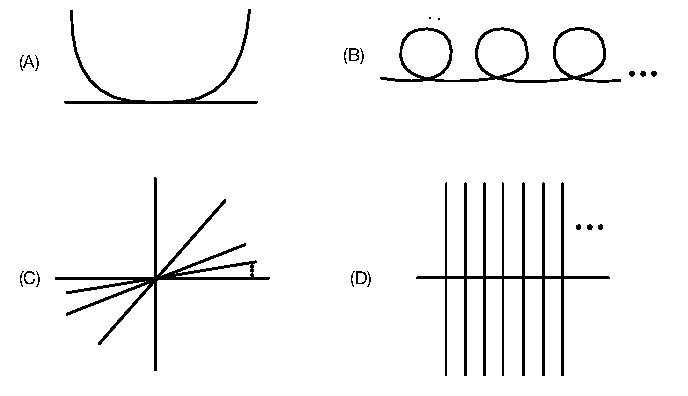
\includegraphics[width=.8\textwidth]{figures/appendix-c-artin-counterexamples.pdf}
\caption{Artin 公理的反例}\bookfigurehref{C.7.16}\label{src:C.7.16}
\end{figure}
\begin{example}[无限相切的曲线]\label{src:C.7.17}
对于图 \hyperref[src:C.7.16]{3.7.16}(A), 令 $X_q=\Spec A_q$, 其中 $A_q=\Bbbk[x,y]/(y(y-x^q))$, $A_{q+1}\to A_q$ 由 $(x,y)\mapsto(x,xy)$ 定义. 在 $F(\Bbbk[t]/t^{n+1})$ 中, 考虑由 $(x,y)\mapsto(t,0)$ 定义的元素 $\alpha_n:A_q\to\Bbbk[t]/t^{n+1}$ (对任何 $q$), 以及由 $(x,y)\mapsto(t,t^q)$ 定义的 $\beta_n:A_q\to\Bbbk[t]/t^{n+1}$ (对任何 $q$). 对每个 $n$, $\alpha_n\sim\beta_n$, 因为可取 $q\geq n+1$. 于是 $\{\alpha_n\}$ 是万有形式形变, 可有效化为两个不同的元素 $\widehat\alpha,\widehat\beta\in F(\Bbbk[\![t]\!])$, 它们在 $A_q$ (对任何 $q$) 上分别由 $\widehat\alpha(x,y)\mapsto(t,0)$ 与 $\widehat\beta(x,y)\mapsto(t,t^q)$ 定义. 因而函子 $F(\Bbbk[t])\to\varprojlim F(\Bbbk[t]/t^q)$ 不单射, 所以有效性公理 $(\mathrm{AA}_5)$ 不成立. 此时 \bookref{C.7.1}(5) (万有性的开性) 也不成立. 同样, $F$ 的对角不可表: $\underline{\Isom}_{\Bbbk[t]}(\widehat\alpha,\widehat\beta)$ 的形式形变 $\{\alpha_n\xrightarrow\sim\beta_n\}$ 无效.
\end{example}
\begin{example}[无限多个节点]\label{src:C.7.18}
对于图 \hyperref[src:C.7.16]{3.7.16}(B), 令 $X_q$ 为将 $\mathbb A^1$ 上 $q$ 对点按节点方式粘合得到的具有 $q$ 个节点的 $\mathbb C$ 上仿射概形. 则 $\mathbb A^1\to\operatorname{colim}X_q$ 在任何不映到节点的点处形式万有, 但在 $\mathbb A^1$ 的任何开邻域中都不形式万有, 因为必须去掉无限多个点. 因而 \bookref{C.7.1}(5) (万有性的开性) 不成立.

类似地, 对于图 \hyperref[src:C.7.16]{3.7.16}(C), 若 $X_q=\Spec\Bbbk[x,y]/(y\prod_{i=1}^1(x-q))$, 则包含映射 $\mathbb A^1\to\operatorname{colim}X_q$ 在任何非节点处形式万有, 但在开邻域中不形式万有.
\end{example}
\begin{example}[无限多条直线]\label{src:C.7.19}
对于图 \hyperref[src:C.7.16]{3.7.16}(D), 令 $X_q=\Spec\Bbbk[x,y]/\prod_{i=1}^q(iy-x)$ 为平面中 $q$ 条直线的并, $X_q\to X_{q+1}$ 为诱导的闭浸入. 则 $\operatorname{colim}X_q$ 满足 Schlessinger 公理 $(\mathrm H_1)$--$(\mathrm H_4)$ (等价地, Rim--Schlessinger 公理 $(\mathrm{RS}_1)$--$(\mathrm{RS}_4)$). 因而可应用 Schlessinger 定理得到形式万有形变 $\{x_n\}$, 其中 $x_n\in(\operatorname{colim}X_q)(\Bbbk[x,y]/(x,y)^{n+1})$ 由闭浸入 $\Spec\Bbbk[x,y]/(x,y)^{n+1}\to X_{n+1}$ 定义. 有效性公理 $(\mathrm{AA}_5)$ 不成立, 因为不存在延拓 $\{x_n\}$ 的 $(\operatorname{colim}X_q)(\Bbbk[x,y])$ 的元素.
\end{example}
\begin{example}[Hom 叠]\label{src:C.7.20}
若 $\mathcal X,\mathcal Y$ 在 $\Bbbk$ 上固有, 则 $(\Sch/\Bbbk)_{\text{ét}}$ 上的 Hom 叠 $\underline{\operatorname{Mor}}(\mathcal X,\mathcal Y)$ 是代数叠 (习题 \bookref{C.7.9}). 更一般地, 对任意基底, 若 $\mathcal X\to S$ 固有且平坦, 而只假设 $\mathcal Y\to S$ 局部有限表现, 拟分离且稳定子群仿射, 结论仍成立; 见 \cite[定理 $1.2$]{HR19b} 和 \cite[推论 $1.6$]{BHL17}. 在这些情形中, Tannaka 对偶 (\bookref{7.6.1}) 的一个版本成立, 即 $\operatorname{Mor}(\mathcal X,\mathcal Y)\xrightarrow\sim\operatorname{Mor}^{\otimes}(\operatorname{Coh}(\mathcal Y),\operatorname{Coh}(\mathcal X))$, 从而将有效性公理 $(\mathrm{AA}_5)$ 归结为 Grothendieck 存在性定理的一个版本.

然而, $\mathcal Y$ 具有仿射稳定子至关重要. 若 $\mathcal Y$ 为阿贝尔簇的分类叠, 则 Tannaka 对偶可能不成立, Hom 叠 $\underline{\operatorname{Mor}}(\mathcal X,\mathcal Y)$ 可能不是代数叠; 见 \cite[Tag 0AF8]{SP} 和 \cite[\S$10$]{HR19b}.
\end{example}
\begin{exercise}[光滑曲线函子的层化]\label{src:C.7.21}
设 $F$ 为函子 $S\mapsto\mathcal M_g(S)/{\sim}$ 在 $(\Sch/\Bbbk)_{\text{ét}}$ 中的层化, 其中 $\mathcal M_g(S)/{\sim}$ 为 $S$ 上光滑曲线族的同构类集合. $F$ 不满足哪一条 Artin 公理?
\end{exercise}
